
% ════════════════════════════════════════════
% 模型准备（5.4.2.模型准备.tex，三级子块）
% ════════════════════════════════════════════
\subsubsection{波动电价数据的处理}

\textbf{1.数据预处理}

附件四给出 2025 年全年逐 10 分钟的外网实时波动电价。记第 $d$ 天第 $k$ 个间隔的波动电价为 $p_{d,k}$，全年电价数据可组织为
\begin{equation}
    \boldsymbol{P}=[p_{d,k}]_{365\times 144}
\end{equation}
全年无缺失值，电价分布范围约为 $0.3\sim 1.6$ 元/kWh。波动电价与固定电价的典型日对比如图\ref{fig:preprocess4}所示。

\begin{figure}[H]
    \centering
    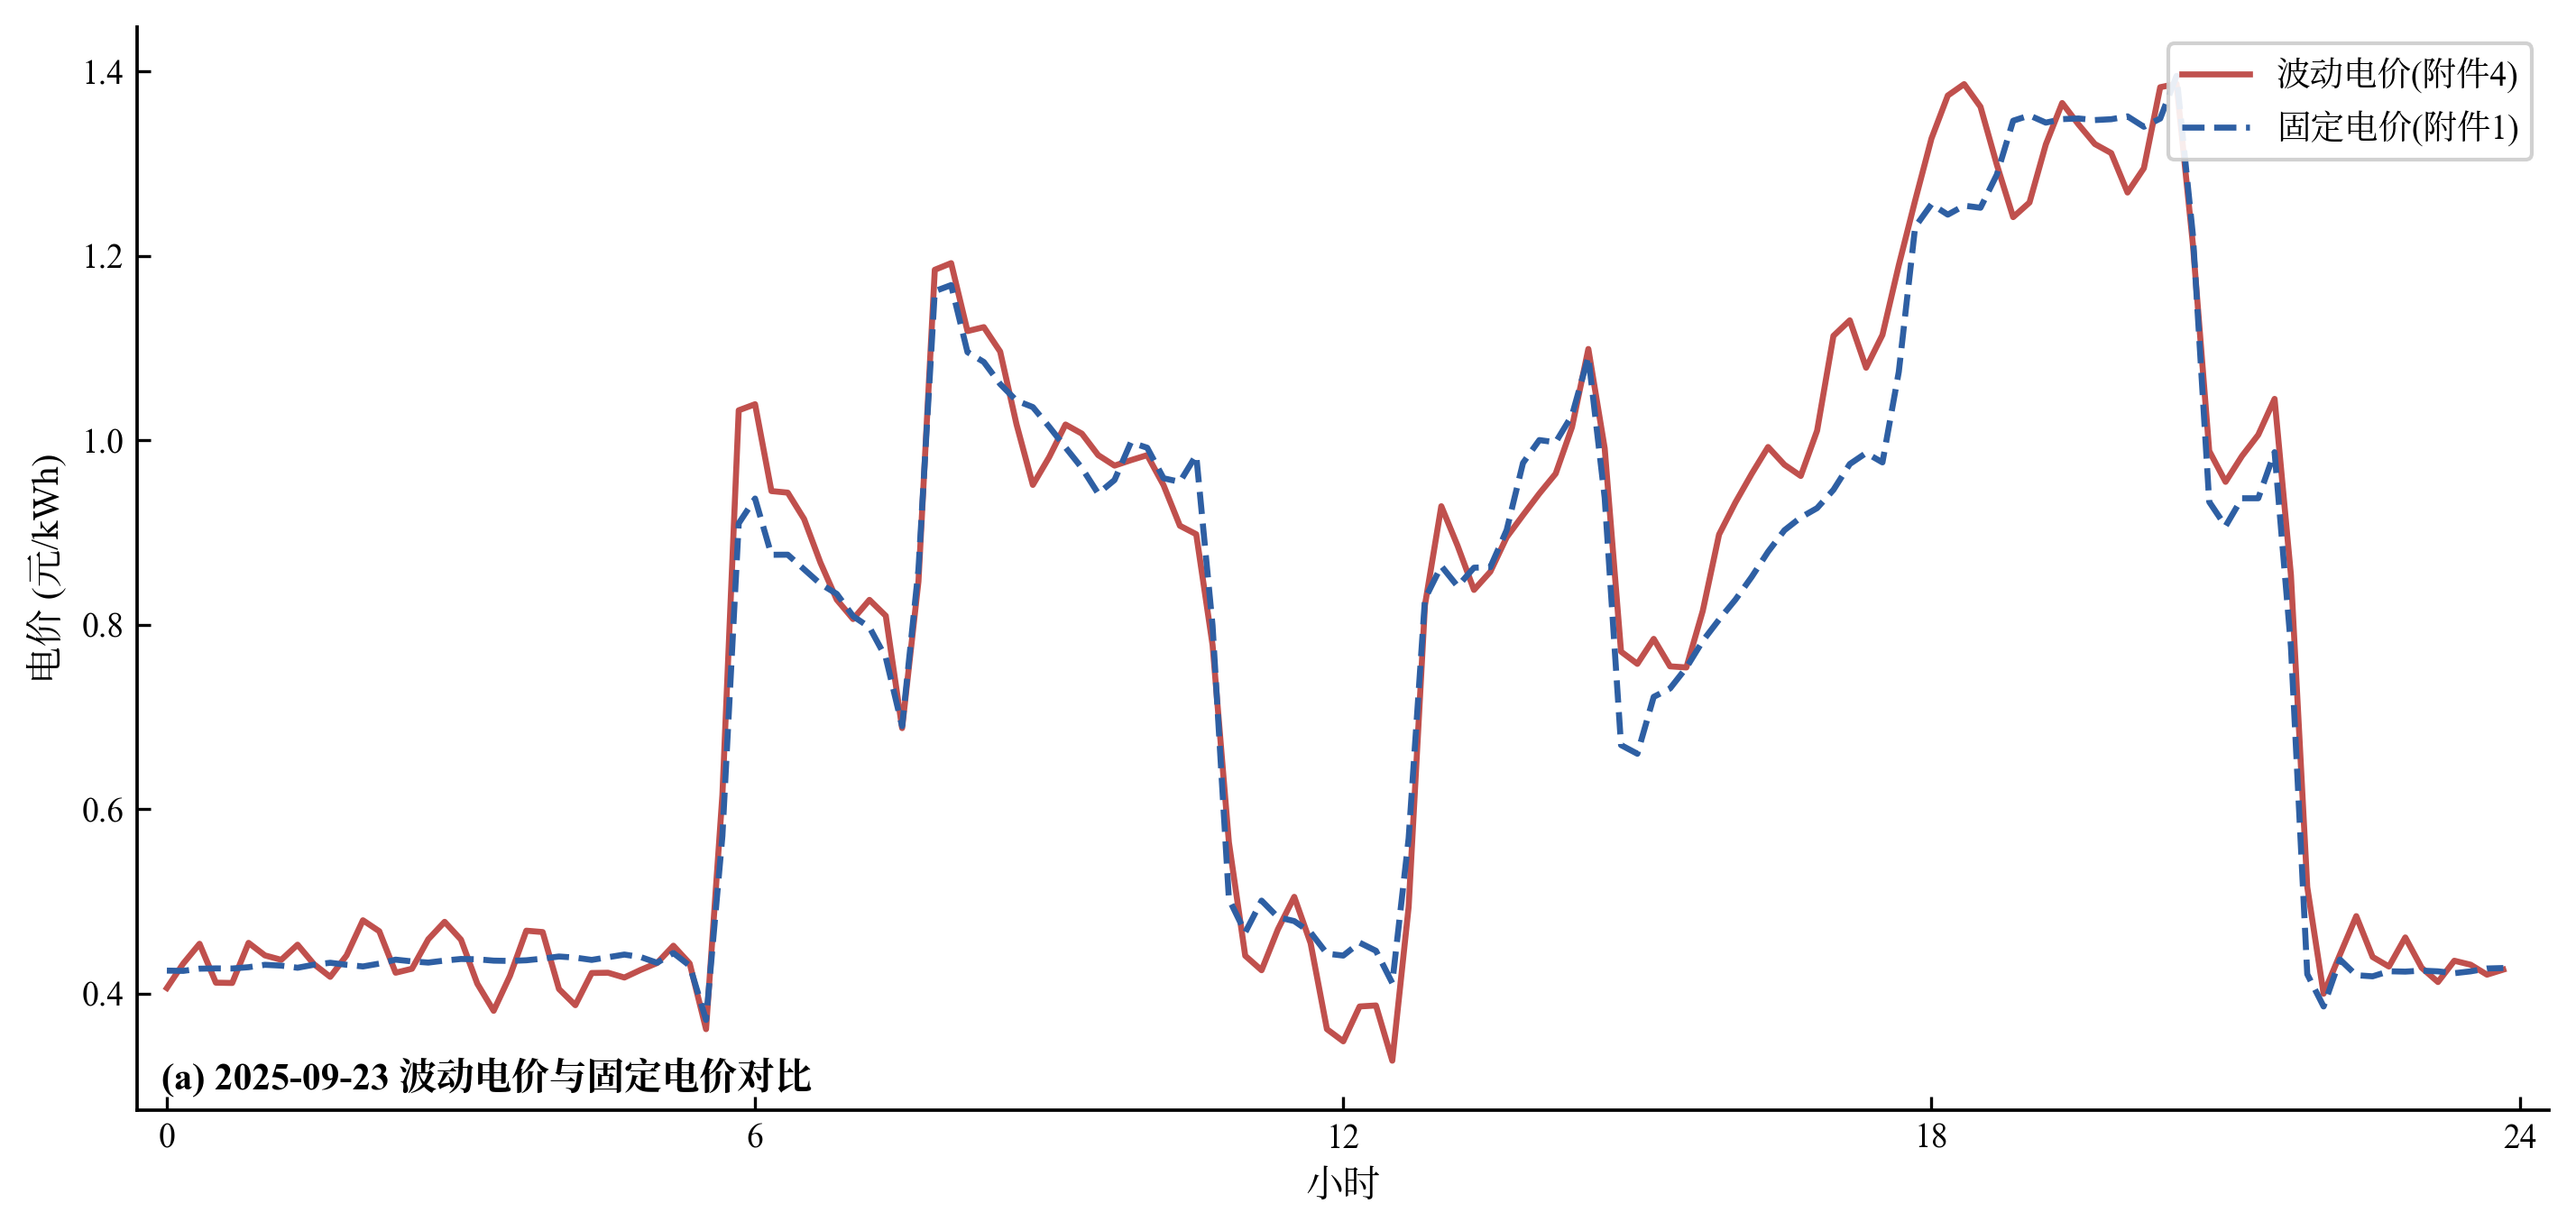
\includegraphics[width=0.46\textwidth]{求解/问题四/图片/图4-1_波动与固定电价对比.png}
    \caption{波动电价与固定电价的典型日对比}
    \label{fig:preprocess4}
\end{figure}

图\ref{fig:preprocess4}中，波动电价在一天内剧烈起伏，白天高峰可达 1.5 元/kWh 以上，夜间低谷低至 0.35 元/kWh 左右，峰谷价差明显大于固定电价，储能低充高放的套利空间更大，购电时机的把握也更关键。

\textbf{2.算法选择}

本问建模框架与问题二、问题三一致，目标函数与约束均为线性：问题二对应部分用逐日线性规划，问题三对应部分用滚动线性规划，只需把电价参数 $p_k$ 替换为 $p_{d,k}$。
